\chapter{Latex Usage}
\label{chapter:latexUsage}
\graphicspath{ {./chapter01/Fig} }

\begin{itquote}
The journey of a thousand miles begins with one step.
\end{itquote}

I can't be the only one.  I say this as I struggle to convert a textbook written
in Microsoft Word to Latex and post it on GitHub.  There must be others like me
with quality content they've created for their classes that they want to share.
So this text is an Open Education Resources, free to use under the Creative
Commons license.  But how can we take advantage of deep reservoir of 
knowledge the community of senior design faculty have created over the
years.   In taking this particular project on, I want to move a step
towards the solution.

By hosting this textbook on Github, I want to encourage others to contribute 
their insights and ideas into our text.  For example, some of the processes in
this text are outdated. If that annoys you, then go to the
\url{https://github.com/coulston/Design-For-Electrical-and-Computer-Engineering}
{textbook repository} fork, clone, make a branch, make your changes and
then do a pull request to merge them into the existing text.  If that sounds a 
bit overwhelming, don't worry, I plan on writing a chapter 2 to this how-to
to walk you through it.  The world is an imperfect place, I want you to be 
empowered to make it better.

\section*{Learning Objectives}
\noindent\rule{\linewidth}{1pt}
By the end of this chapter, the reader should:
\begin{itemize}
\item 	Understand some of my motivations in this project.
\item 	Understand the general philosophy of writing Latex for this text.
\item Know how to create common structures like table, figure, examples.
\item Know how to use the Example environment.
\item Know how to create references to structures.
\end{itemize}

\section{Table}
\label{section:the-first-section}
When deciding on a methodology to implement some text formatting question,
my preference is to work with the existing LaTex packages before adding new
packages because every additional package adds additional time to build the
text.  All things being equal, I will always prefer a Minimum Working Example 
(MWE) over something more complex.  As a consequence of these two preferences,
when you inevitably need to search for a way to complete some text formatting
goal, I generally preface "MWE" in front of the thing I am trying to accomplish.

While tables are an incredibly important tool to communicate a lot of information 
in a structured format, they can be a challenge to tame.  As a result, I'll introduce
Table~\ref{table:thisIsTheFirstTable} as an example.  The Latex code for this table
is shown below.


\begin{verbatim}
\begin{table}[h]
\caption{This is an important table.}
\label{table:thisIsTheFirstTable}
\begin{tabular}{|g|c|c|c|c|}
\hline
\rowcolor{Gray}
 & & \multicolumn{3} {c|} {Alternatives} \\ \hhline{|~|~|-|-|-|}
\rowcolor{Gray}
 \multirow{-2}{*}{Selection Criteria} & \multirow{-2}{*}{Weights}  & Project 1 & Project 2 & Project 3 \\ \hline
A (Match to skills) & 0.52 & 0.40 & 0.20 & 0.40 \\  \hline
B (Technical Complexity) & 0.12 & 0.40 & 0.30 & 0.30 \\ \hline
C (Creativity) & 0.09 & 0.45 & 0.20 & 0.35 \\ \hline
D (Market potential) & 0.18 & 0.05 & 0.35 & 0.60 \\ \hline
E (Industry sponsorship) & 0.09 & 0.00 & 1.0 & 0.00 \\ \hline
Score & & 0.31 & 0.31 & 0.38 \\ \hline
\end{tabular}
\end{table}
\end{verbatim}

There are several packages that will make this table look non-standard.  
\begin{enumerate}
\item \begin{verbatim} \rowcolor{Gray} \end{verbatim}
\item \
\end{\begin{verbatim}

\begin{table}[h]
\caption{This is an important table.}
\label{table:thisIsTheFirstTable}
\begin{tabular}{|l|c|c|c|c|}
\hline
\rowcolor{Gray}
 & & \multicolumn{3} {c|} {Alternatives} \\ \hhline{|~|~|-|-|-|}
\rowcolor{Gray}
 \multirow{-2}{*}{Selection Criteria} & \multirow{-2}{*}{Weights}  & Project 1 & Project 2 & Project 3 \\ \hline
A (Match to skills) & 0.52 & 0.40 & 0.20 & 0.40 \\  \hline
B (Technical Complexity) & 0.12 & 0.40 & 0.30 & 0.30 \\ \hline
C (Creativity) & 0.09 & 0.45 & 0.20 & 0.35 \\ \hline
D (Market potential) & 0.18 & 0.05 & 0.35 & 0.60 \\ \hline
E (Industry sponsorship) & 0.09 & 0.00 & 1.0 & 0.00 \\ \hline
Score & & 0.31 & 0.31 & 0.38 \\ \hline
\end{tabular}
\end{table}


\lipsum[9]
A reference to Figure~\ref{figure:dilbertCommunication}.
\lipsum[10]

\begin{figure}[h]
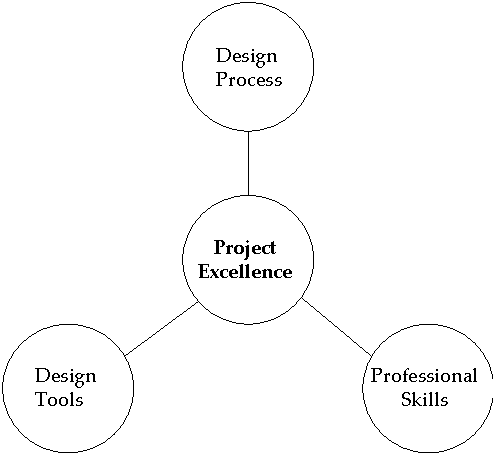
\includegraphics[width=5.5in,height=1.9in]{image7}
\caption{The dimensions of the engineering design process according to Ford and Coulston.)}
\label{figure:engineeringDimensions}
\end{figure}


\lipsum[11]
A reference to Equation~\ref{equ:simpleEquation}.
\lipsum[12]


\begin{equation}
\label{equ:simpleEquation}
x = \int v(t) dt
\end{equation}

\lipsum[12]

\begin{example}{A Simple Example}
\label{example:aSimpleExample}
\emph{\textbf{\ul{Problem:}}} Consider.... \\	% Force line break for spacing
\noindent\emph{\textbf{\ul{Solution:}}} The parallel systems...
\end{example}

\lipsum[13]

\begin{itemize}
\item
  US Bureau of Labor Statistics, \url{http://stats.bls.gov}.
  different industry sectors.
\item
  US Government Official WebPortal,  \href{http://www.FirstGov.gov}{www.FirstGov.gov}. 
\item
  US Patent Office, \href{http://www.uspto.gov}{www.uspto.gov}. A
  searchable database of all patents back to 1790. 
\end{itemize}



\section{Summary and Further Reading}
\label{section:summary-and-further-reading}

\lipsum[30-31]
